
Write and run a computer program to estimate $\mathbb{E}_\pi[(X_1-X_2)/(1+X_3+X_4X_5)]$ using an MCMC algorithm of your choice, and obtain the best estimate you can. Include some discussion of accuracy, uncertainty, standard errors, etc.\\

For this problem, we will use a Random Walk Metropolis algorithm to estimate the expectation. The increments in the random walk follow a $N(0,\sigma^2 I)$ distribution, where we will set the parameter $\sigma=0.2$ (by trial and error to minimize se).\\

Source code:
\begin{knitrout}
\definecolor{shadecolor}{rgb}{0.969, 0.969, 0.969}\color{fgcolor}\begin{kframe}
\begin{alltt}
\hlcom{#Estimate E_pi((X1-X2)/(1+X3+X4X5)) where pi=cg using RWM algorithm }
\hlcom{# with increments following a N(0,sigma^2*I) distribution}

\hlstd{A} \hlkwb{=} \hlnum{7}\hlstd{; B} \hlkwb{=} \hlnum{6}\hlstd{; C} \hlkwb{=} \hlnum{6}\hlstd{; D} \hlkwb{=} \hlnum{3}

\hlstd{fn} \hlkwb{=} \hlkwa{function}\hlstd{(}\hlkwc{x1}\hlstd{,}\hlkwc{x2}\hlstd{,}\hlkwc{x3}\hlstd{,}\hlkwc{x4}\hlstd{,}\hlkwc{x5}\hlstd{) \{(x1}\hlopt{-}\hlstd{x2)}\hlopt{/}\hlstd{(}\hlnum{1}\hlopt{+}\hlstd{x3}\hlopt{+}\hlstd{x4}\hlopt{*}\hlstd{x5)\}}
\hlstd{g} \hlkwb{=} \hlkwa{function}\hlstd{(}\hlkwc{x1}\hlstd{,}\hlkwc{x2}\hlstd{,}\hlkwc{x3}\hlstd{,}\hlkwc{x4}\hlstd{,}\hlkwc{x5}\hlstd{) \{}
  \hlkwa{if} \hlstd{(x1}\hlopt{<=}\hlnum{0} \hlopt{|} \hlstd{x1}\hlopt{>=}\hlnum{2} \hlopt{|} \hlstd{x2}\hlopt{<=}\hlnum{0} \hlopt{|} \hlstd{x2}\hlopt{>=}\hlnum{2} \hlopt{|}\hlstd{x3}\hlopt{<=}\hlnum{0} \hlopt{|} \hlstd{x3}\hlopt{>=}\hlnum{2} \hlopt{|}
      \hlstd{x4}\hlopt{<=}\hlnum{0} \hlopt{|} \hlstd{x4}\hlopt{>=}\hlnum{2} \hlopt{|} \hlstd{x5}\hlopt{<=}\hlnum{0} \hlopt{|} \hlstd{x5}\hlopt{>=}\hlnum{2}\hlstd{)}
    \hlnum{0}
  \hlkwa{else}
    \hlstd{(x1}\hlopt{+}\hlstd{A}\hlopt{+}\hlnum{2}\hlstd{)}\hlopt{^}\hlstd{(x2}\hlopt{+}\hlnum{3}\hlstd{)}\hlopt{*}\hlstd{(}\hlnum{1}\hlopt{+}\hlkwd{cos}\hlstd{((B}\hlopt{+}\hlnum{3}\hlstd{)}\hlopt{*}\hlstd{x3))}\hlopt{*}\hlstd{(}\hlkwd{exp}\hlstd{((}\hlnum{12}\hlopt{-}\hlstd{C)}\hlopt{*}\hlstd{x4))}\hlopt{*}\hlkwd{abs}\hlstd{(x4}\hlopt{-}\hlnum{3}\hlopt{*}\hlstd{x5)}\hlopt{^}\hlstd{(D}\hlopt{+}\hlnum{2}\hlstd{)}
\hlstd{\}}

\hlstd{sigma} \hlkwb{=} \hlnum{0.2}
\hlstd{M} \hlkwb{=} \hlnum{1e+6}
\hlstd{B} \hlkwb{=} \hlnum{1e+5}

\hlcom{#initialization}
\hlstd{fnlist} \hlkwb{=} \hlkwd{numeric}\hlstd{(M}\hlopt{+}\hlstd{B)}
\hlstd{x1} \hlkwb{=} \hlkwd{runif}\hlstd{(}\hlnum{1}\hlstd{,}\hlnum{0}\hlstd{,}\hlnum{2}\hlstd{)}
\hlstd{x2} \hlkwb{=} \hlkwd{runif}\hlstd{(}\hlnum{1}\hlstd{,}\hlnum{0}\hlstd{,}\hlnum{2}\hlstd{)}
\hlstd{x3} \hlkwb{=} \hlkwd{runif}\hlstd{(}\hlnum{1}\hlstd{,}\hlnum{0}\hlstd{,}\hlnum{2}\hlstd{)}
\hlstd{x4} \hlkwb{=} \hlkwd{runif}\hlstd{(}\hlnum{1}\hlstd{,}\hlnum{0}\hlstd{,}\hlnum{2}\hlstd{)}
\hlstd{x5} \hlkwb{=} \hlkwd{runif}\hlstd{(}\hlnum{1}\hlstd{,}\hlnum{0}\hlstd{,}\hlnum{2}\hlstd{)}
\hlstd{acc} \hlkwb{=} \hlnum{0}

\hlkwa{for} \hlstd{(i} \hlkwa{in} \hlnum{1}\hlopt{:}\hlstd{(M}\hlopt{+}\hlstd{B)) \{}
  \hlstd{eps} \hlkwb{=} \hlkwd{rnorm}\hlstd{(}\hlnum{5}\hlstd{,}\hlnum{0}\hlstd{,sigma)}

  \hlkwa{if} \hlstd{(}\hlkwd{runif}\hlstd{(}\hlnum{1}\hlstd{)}\hlopt{<=}\hlkwd{g}\hlstd{(x1}\hlopt{+}\hlstd{eps[}\hlnum{1}\hlstd{],x2}\hlopt{+}\hlstd{eps[}\hlnum{2}\hlstd{],x3}\hlopt{+}\hlstd{eps[}\hlnum{3}\hlstd{],x4}\hlopt{+}\hlstd{eps[}\hlnum{4}\hlstd{],x5}\hlopt{+}\hlstd{eps[}\hlnum{5}\hlstd{])}\hlopt{/}
        \hlkwd{g}\hlstd{(x1,x2,x3,x4,x5)) \{}
    \hlkwa{if} \hlstd{(i}\hlopt{>}\hlstd{B)}
      \hlstd{acc}\hlkwb{=}\hlstd{acc}\hlopt{+}\hlnum{1}
    \hlstd{x1}\hlkwb{=}\hlstd{x1}\hlopt{+}\hlstd{eps[}\hlnum{1}\hlstd{]}
    \hlstd{x2}\hlkwb{=}\hlstd{x2}\hlopt{+}\hlstd{eps[}\hlnum{2}\hlstd{]}
    \hlstd{x3}\hlkwb{=}\hlstd{x3}\hlopt{+}\hlstd{eps[}\hlnum{3}\hlstd{]}
    \hlstd{x4}\hlkwb{=}\hlstd{x4}\hlopt{+}\hlstd{eps[}\hlnum{4}\hlstd{]}
    \hlstd{x5}\hlkwb{=}\hlstd{x5}\hlopt{+}\hlstd{eps[}\hlnum{5}\hlstd{]}
  \hlstd{\}}
  \hlstd{fnlist[i]} \hlkwb{=} \hlkwd{fn}\hlstd{(x1,x2,x3,x4,x5)}
\hlstd{\}}

\hlstd{funcmean} \hlkwb{=} \hlkwd{mean}\hlstd{(fnlist[(B}\hlopt{+}\hlnum{1}\hlstd{)}\hlopt{:}\hlstd{(M}\hlopt{+}\hlstd{B)])}
\hlstd{funciidse} \hlkwb{=} \hlkwd{sd}\hlstd{(fnlist[(B}\hlopt{+}\hlnum{1}\hlstd{)}\hlopt{:}\hlstd{(M}\hlopt{+}\hlstd{B)])}\hlopt{/}\hlkwd{sqrt}\hlstd{(M)}
\hlstd{acf_k} \hlkwb{=} \hlkwd{acf}\hlstd{(fnlist[(B}\hlopt{+}\hlnum{1}\hlstd{)}\hlopt{:}\hlstd{(M}\hlopt{+}\hlstd{B)],}\hlkwc{lag.max} \hlstd{=} \hlnum{1000}\hlstd{,}\hlkwc{plot} \hlstd{=} \hlnum{FALSE}\hlstd{)}\hlopt{$}\hlstd{acf}
\hlstd{varfact} \hlkwb{=} \hlnum{2}\hlopt{*}\hlkwd{sum}\hlstd{(acf_k[}\hlnum{1}\hlopt{:}\hlkwd{min}\hlstd{(}\hlkwd{which}\hlstd{(acf_k}\hlopt{<}\hlnum{0.05}\hlstd{))])}\hlopt{-}\hlnum{1}
\hlstd{funcse} \hlkwb{=} \hlstd{funciidse}\hlopt{*}\hlkwd{sqrt}\hlstd{(varfact)}
\hlstd{accrate} \hlkwb{=} \hlstd{acc}\hlopt{/}\hlstd{M}

\hlkwd{cat}\hlstd{(}\hlstr{'B = '}\hlstd{,B,}\hlstr{', M = '}\hlstd{,M,}\hlstr{'\textbackslash{}n'}\hlstd{)}
\hlkwd{cat}\hlstd{(}\hlstr{'Number of samples accepted = '}\hlstd{,acc,}\hlstr{', acceptance rate = '}\hlstd{,accrate,}\hlstr{'\textbackslash{}n'}\hlstd{)}
\hlkwd{cat}\hlstd{(}\hlstr{'Estimate = '}\hlstd{,funcmean,}\hlstr{'\textbackslash{}n'}\hlstd{)}
\hlkwd{cat}\hlstd{(}\hlstr{'i.i.d. standard error = '}\hlstd{,funciidse,}\hlstr{'\textbackslash{}n'}\hlstd{)}
\hlkwd{cat}\hlstd{(}\hlstr{'varfact = '}\hlstd{,varfact,}\hlstr{'\textbackslash{}n'}\hlstd{)}
\hlkwd{cat}\hlstd{(}\hlstr{'Standard error = '}\hlstd{,funcse,}\hlstr{'\textbackslash{}n'}\hlstd{)}
\end{alltt}
\end{kframe}
\end{knitrout}
Output of several runs:
\begin{knitrout}
\definecolor{shadecolor}{rgb}{0.969, 0.969, 0.969}\color{fgcolor}\begin{kframe}
\begin{verbatim}
## B =  1e+05 , M =  1e+06 
## Number of samples accepted =  173759 , acceptance rate =  0.173759 
## Estimate =  -0.08263961 
## i.i.d. standard error =  0.000135386 
## varfact =  175.5155 
## Standard error =  0.001793624
## B =  1e+05 , M =  1e+06 
## Number of samples accepted =  173366 , acceptance rate =  0.173366 
## Estimate =  -0.08711674 
## i.i.d. standard error =  0.0001361279 
## varfact =  183.7932 
## Standard error =  0.001845491
## B =  1e+05 , M =  1e+06 
## Number of samples accepted =  173740 , acceptance rate =  0.17374 
## Estimate =  -0.08693576 
## i.i.d. standard error =  0.0001343732 
## varfact =  172.7299 
## Standard error =  0.001766024
## B =  1e+05 , M =  1e+06 
## Number of samples accepted =  173184 , acceptance rate =  0.173184 
## Estimate =  -0.08750525 
## i.i.d. standard error =  0.0001351836 
## varfact =  175.3872 
## Standard error =  0.001790288
## B =  1e+05 , M =  1e+06 
## Number of samples accepted =  172432 , acceptance rate =  0.172432 
## Estimate =  -0.08019379 
## i.i.d. standard error =  0.0001348094 
## varfact =  182.1287 
## Standard error =  0.001819321
\end{verbatim}
\end{kframe}
\end{knitrout}
The tabulated result is as follows:\\
\begin{center}
\begin{knitrout}
\definecolor{shadecolor}{rgb}{0.969, 0.969, 0.969}\color{fgcolor}
\begin{tabular}{r|r|r|r|r}
\hline
estimation & acc\_rate & seiid & varfact & standard\_error\\
\hline
-0.0826396 & 0.173759 & 0.0001354 & 182.1287 & 0.0017936\\
\hline
-0.0871167 & 0.173366 & 0.0001361 & 182.1287 & 0.0018455\\
\hline
-0.0869358 & 0.173740 & 0.0001344 & 182.1287 & 0.0017660\\
\hline
-0.0875052 & 0.173184 & 0.0001352 & 182.1287 & 0.0017903\\
\hline
-0.0801938 & 0.172432 & 0.0001348 & 182.1287 & 0.0018193\\
\hline
\end{tabular}


\end{knitrout}
\end{center}
From the table above, we can first notice that the estimated result is consistent with the previous samplers, but the range of the estimation is slightly larger here using the MCMC sampler, while the standard error is smaller in this case. Also, we see that the acceptance rate is about 17\%, and is close the the optimal 23\%. To verify that the MCMC sampler works effectively, we plot the value of the estimated function after the burn-in stage
\begin{figure}[H]
  \centering
\begin{knitrout}
\definecolor{shadecolor}{rgb}{0.969, 0.969, 0.969}\color{fgcolor}\begin{kframe}
\begin{alltt}
\hlstd{fnlist6} \hlkwb{=} \hlstd{fnlist}
\hlkwd{plot}\hlstd{(fnlist6[(B}\hlopt{+}\hlnum{1}\hlstd{)}\hlopt{:}\hlstd{(B}\hlopt{+}\hlstd{M)],}\hlkwc{type}\hlstd{=}\hlstr{'l'}\hlstd{)}
\end{alltt}
\end{kframe}
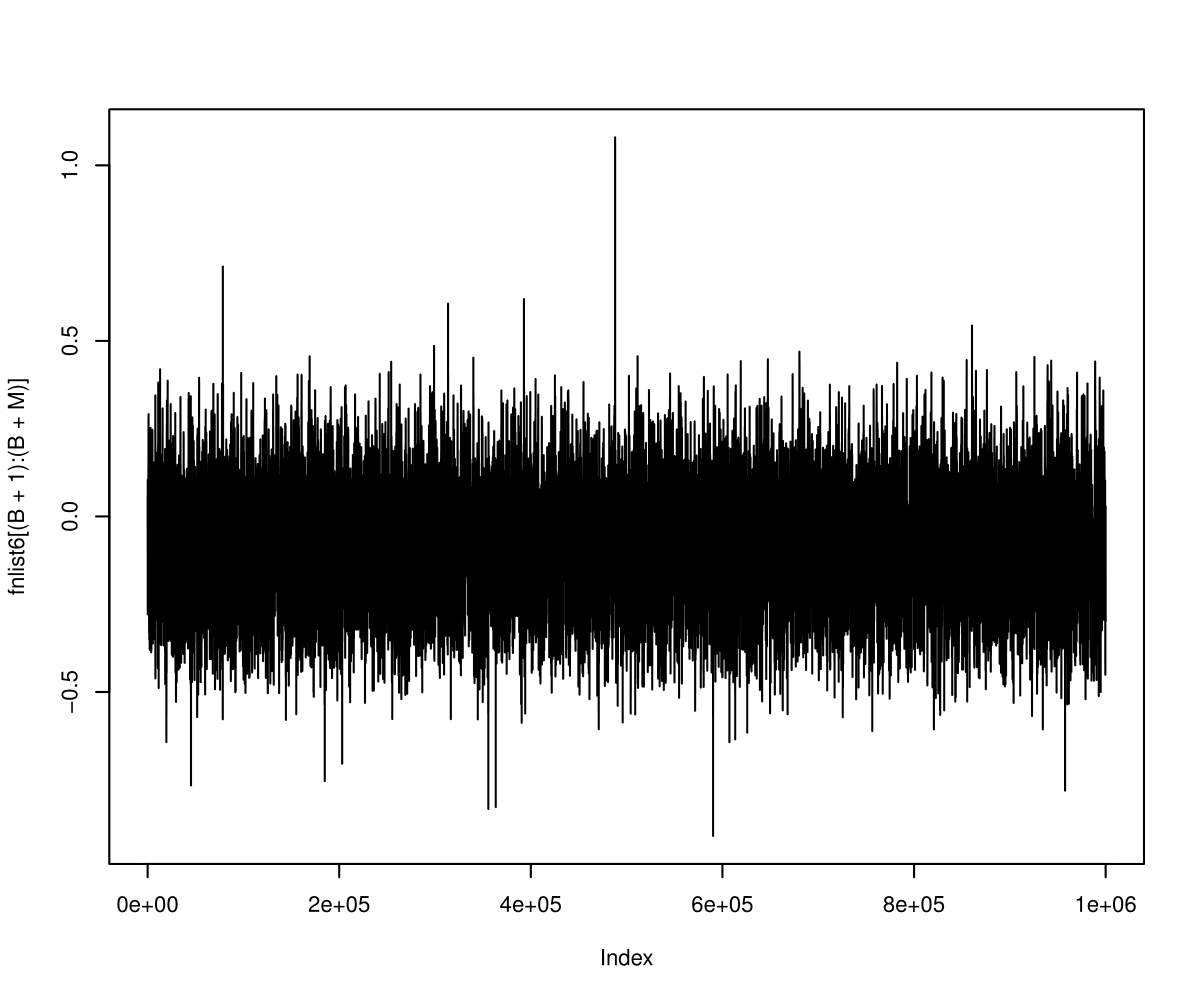
\includegraphics[width=\maxwidth]{figure/p6plot-1} 

\end{knitrout}
		\caption{function values of MCMC algorithm after burning-in}
\end{figure}

From the figure above, we can see that the sample is reasonably well represented (at least the value of the function itself varies significantly around its mean value), indicating a good (accurate) approximation by the MCMC algorithm.
